\documentclass[varwidth=16cm,border=10pt]{standalone}

% Use [preprint] to show author names for your class paper. 
% Use [final] for camera-ready. 
% If you remove the option, it defaults to anonymous submission.

\usepackage[utf8]{inputenc} % allow utf-8 input
\usepackage[T1]{fontenc}    % use 8-bit T1 fonts
\usepackage{hyperref}       % hyperlinks
\usepackage{url}            % simple URL typesetting
\usepackage{booktabs}       % professional-quality tables
\usepackage{amsfonts}       % blackboard math symbols
\usepackage{nicefrac}       % compact symbols for 1/2, etc.
\usepackage{microtype}      % microtypography
\usepackage{graphicx}       % for images
\usepackage{float}          % for [H] in algorithms
\usepackage{subcaption}
\usepackage{xcolor}
\usepackage{tikz}
\usetikzlibrary{shapes.misc}
\usetikzlibrary{positioning}
\usepackage{float}

% Algorithm packages
\usepackage[ruled,vlined,linesnumbered]{algorithm2e}

% Math packages
\usepackage{amsmath}
\usepackage{amsthm}
\usepackage{amssymb}
\usepackage{bm}
\usepackage{dsfont} % for \mathds
\usepackage{enumitem}

\usetikzlibrary{shapes.geometric, arrows.meta, positioning, patterns, calc, fit, decorations.pathreplacing, shadows}

% --- MACROS START ---

% Standard definitions
\DeclareMathOperator*{\argmin}{argmin}
\DeclareMathOperator*{\argmax}{argmax}
\DeclareMathOperator*{\minimize}{minimize}
\DeclareMathOperator{\sign}{sign}
\DeclareMathOperator{\tr}{tr}
\DeclareMathOperator{\Var}{Var}
\DeclareMathOperator*{\Cor}{Corr}
\DeclareMathOperator*{\Cov}{Cov}
\DeclareMathOperator*{\ind}{\mathds{1}}

\theoremstyle{definition}
\newtheorem{definition}{Definition}
\newtheorem{notation}[definition]{Notation}
\newtheorem{proposition}[definition]{Proposition}
\newtheorem{theorem}[definition]{Theorem}

% Bold fonts
\newcommand{\ab}{\mathbf{a}}
\newcommand{\bbb}{\mathbf{b}}
\newcommand{\cbb}{\mathbf{c}}
\newcommand{\db}{\mathbf{d}}
\newcommand{\eb}{\mathbf{e}}
\newcommand{\fb}{\mathbf{f}}
\newcommand{\gb}{\mathbf{g}}
\newcommand{\hb}{\mathbf{h}}
\newcommand{\ib}{\mathbf{i}}
\newcommand{\jb}{\mathbf{j}}
\newcommand{\kb}{\mathbf{k}}
\newcommand{\lb}{\mathbf{l}}
\newcommand{\mb}{\mathbf{m}}
\newcommand{\nbb}{\mathbf{n}}
\newcommand{\ob}{\mathbf{o}}
\newcommand{\pb}{\mathbf{p}}
\newcommand{\qb}{\mathbf{q}}
\newcommand{\rb}{\mathbf{r}}
\newcommand{\sbb}{\mathbf{s}}
\newcommand{\tb}{\mathbf{t}}
\newcommand{\ub}{\mathbf{u}}
\newcommand{\vb}{\mathbf{v}}
\newcommand{\wb}{\mathbf{w}}
\newcommand{\xb}{\mathbf{x}}
\newcommand{\yb}{\mathbf{y}}
\newcommand{\zb}{\mathbf{z}}

\newcommand{\ba}{\bm{a}}
\newcommand{\bb}{\bm{b}}
\newcommand{\bc}{\bm{c}}
\newcommand{\bd}{\bm{d}}
\newcommand{\be}{\bm{e}}
\newcommand{\bbf}{\bm{f}}
\newcommand{\bg}{\bm{g}}
\newcommand{\bh}{\bm{h}}
\newcommand{\bi}{\bm{i}}
\newcommand{\bj}{\bm{j}}
\newcommand{\bk}{\bm{k}}
\newcommand{\bl}{\bm{l}}
\newcommand{\bbm}{\bm{m}}
\newcommand{\bn}{\bm{n}}
\newcommand{\bo}{\bm{o}}
\newcommand{\bp}{\bm{p}}
\newcommand{\bq}{\bm{q}}
\newcommand{\br}{\bm{r}}
\newcommand{\bs}{\bm{s}}
\newcommand{\bt}{\bm{t}}
\newcommand{\bu}{\bm{u}}
\newcommand{\bv}{\bm{v}}
\newcommand{\bw}{\bm{w}}
\newcommand{\bx}{\bm{x}}
\newcommand{\by}{\bm{y}}
\newcommand{\bz}{\bm{z}}

\newcommand{\Ab}{\mathbf{A}}
\newcommand{\Bb}{\mathbf{B}}
\newcommand{\Cb}{\mathbf{C}}
\newcommand{\Db}{\mathbf{D}}
\newcommand{\Eb}{\mathbf{E}}
\newcommand{\Fb}{\mathbf{F}}
\newcommand{\Gb}{\mathbf{G}}
\newcommand{\Hb}{\mathbf{H}}
\newcommand{\Ib}{\mathbf{I}}
\newcommand{\Jb}{\mathbf{J}}
\newcommand{\Kb}{\mathbf{K}}
\newcommand{\Lb}{\mathbf{L}}
\newcommand{\Mb}{\mathbf{M}}
\newcommand{\Nb}{\mathbf{N}}
\newcommand{\Ob}{\mathbf{O}}
\newcommand{\Pb}{\mathbf{P}}
\newcommand{\Qb}{\mathbf{Q}}
\newcommand{\Rb}{\mathbf{R}}
\newcommand{\Sbb}{\mathbf{S}}
\newcommand{\Tb}{\mathbf{T}}
\newcommand{\Ub}{\mathbf{U}}
\newcommand{\Vb}{\mathbf{V}}
\newcommand{\Wb}{\mathbf{W}}
\newcommand{\Xb}{\mathbf{X}}
\newcommand{\Yb}{\mathbf{Y}}
\newcommand{\Zb}{\mathbf{Z}}

\newcommand{\bA}{\bm{A}}
\newcommand{\bB}{\bm{B}}
\newcommand{\bC}{\bm{C}}
\newcommand{\bD}{\bm{D}}
\newcommand{\bE}{\bm{E}}
\newcommand{\bF}{\bm{F}}
\newcommand{\bG}{\bm{G}}
\newcommand{\bH}{\bm{H}}
\newcommand{\bI}{\bm{I}}
\newcommand{\bJ}{\bm{J}}
\newcommand{\bK}{\bm{K}}
\newcommand{\bL}{\bm{L}}
\newcommand{\bM}{\bm{M}}
\newcommand{\bN}{\bm{N}}
\newcommand{\bO}{\bm{O}}
\newcommand{\bP}{\bm{P}}
\newcommand{\bQ}{\bm{Q}}
\newcommand{\bR}{\bm{R}}
\newcommand{\bS}{\bm{S}}
\newcommand{\bT}{\bm{T}}
\newcommand{\bU}{\bm{U}}
\newcommand{\bV}{\bm{V}}
\newcommand{\bW}{\bm{W}}
\newcommand{\bX}{\bm{X}}
\newcommand{\bY}{\bm{Y}}
\newcommand{\bZ}{\bm{Z}}

% Calligraphic fonts
\newcommand{\cA}{\mathcal{A}}
\newcommand{\cB}{\mathcal{B}}
\newcommand{\cC}{\mathcal{C}}
\newcommand{\cD}{\mathcal{D}}
\newcommand{\cE}{\mathcal{E}}
\newcommand{\cF}{\mathcal{F}}
\newcommand{\cG}{\mathcal{G}}
\newcommand{\cH}{\mathcal{H}}
\newcommand{\cI}{\mathcal{I}}
\newcommand{\cJ}{\mathcal{J}}
\newcommand{\cK}{\mathcal{K}}
\newcommand{\cL}{\mathcal{L}}
\newcommand{\cM}{\mathcal{M}}
\newcommand{\cN}{\mathcal{N}}
\newcommand{\cO}{\mathcal{O}}
\newcommand{\cP}{\mathcal{P}}
\newcommand{\cQ}{\mathcal{Q}}
\newcommand{\cR}{\mathcal{R}}
\newcommand{\cS}{{\mathcal{S}}}
\newcommand{\cT}{{\mathcal{T}}}
\newcommand{\cU}{\mathcal{U}}
\newcommand{\cV}{\mathcal{V}}
\newcommand{\cW}{\mathcal{W}}
\newcommand{\cX}{\mathcal{X}}
\newcommand{\cY}{\mathcal{Y}}
\newcommand{\cZ}{\mathcal{Z}}

% Blackboard bold fonts
\newcommand{\EE}{\mathbb{E}}
\newcommand{\VV}{\mathbb{V}}
\newcommand{\II}{\mathbb{I}}
\newcommand{\KK}{\mathbb{K}}
\newcommand{\LL}{\mathbb{L}}
\newcommand{\MM}{\mathbb{M}}
\newcommand{\NN}{\mathbb{N}}
\newcommand{\PP}{\mathbb{P}}
\newcommand{\QQ}{\mathbb{Q}}
\newcommand{\RR}{\mathbb{R}}
\newcommand{\SSS}{\mathbb{S}}
\newcommand{\ZZ}{\mathbb{Z}}
\newcommand{\XX}{\mathbb{X}}
\newcommand{\YY}{\mathbb{Y}}
\newcommand{\OOmega}{\mathbb{\Omega}}

% Bold greek fonts
\newcommand{\balpha}{\bm{\alpha}}
\newcommand{\bbeta}{\bm{\beta}}
\newcommand{\bgamma}{\bm{\gamma}}
\newcommand{\bepsilon}{\bm{\epsilon}}
\newcommand{\bvarepsilon}{\bm{\varepsilon}}
\newcommand{\bzeta}{\bm{\zeta}}
\newcommand{\btheta}{\bm{\theta}}
\newcommand{\bvartheta}{\bm{\vartheta}}
\newcommand{\bkappa}{\bm{\kappa}}
\newcommand{\blambda}{\bm{\lambda}}
\newcommand{\bmu}{\bm{\mu}}
\newcommand{\bnu}{\bm{\nu}}
\newcommand{\bxi}{\bm{\xi}}
\newcommand{\bpi}{\bm{\pi}}
\newcommand{\bvarpi}{\bm{\varpi}}
\newcommand{\brho}{\bm{\varrho}}
\newcommand{\bsigma}{\bm{\sigma}}
\newcommand{\bvarsigma}{\bm{\varsigma}}
\newcommand{\btau}{\bm{\tau}}
\newcommand{\bupsilon}{\bm{\upsilon}}
\newcommand{\bphi}{\bm{\phi}}
\newcommand{\bvarphi}{\bm{\varphi}}
\newcommand{\bchi}{\bm{\chi}}
\newcommand{\bpsi}{\bm{\psi}}
\newcommand{\bomega}{\bm{\omega}}

\newcommand{\bGamma}{\bm{\Gamma}}
\newcommand{\bDelta}{\bm{\Delta}}
\newcommand{\bTheta}{\bm{\Theta}}
\newcommand{\bLambda}{\bm{\Lambda}}
\newcommand{\bXi}{\bm{\Xi}}
\newcommand{\bPi}{\bm{\Pi}}
\newcommand{\bSigma}{\bm{\Sigma}}
\newcommand{\bUpsilon}{\bm{\Upsilon}}
\newcommand{\bPhi}{\bm{\Phi}}
\newcommand{\bPsi}{\bm{\Psi}}
\newcommand{\bOmega}{\bm{\Omega}}

\newcommand{\smallfrac}[2]{{\textstyle \frac{#1}{#2}}}  
\newcommand*{\zero}{{\bm 0}}
\newcommand*{\one}{{\bm 1}}
\newcommand{\diag}{{\rm diag}}

% --- MACROS END ---

\title{CTC Beam Search with CUDA\\
\small 15-418: Parallel Computer Architecture and Programming, Fall 2025}

\author{%
  Benjamin Kleyner \\
  Computer Science Department \\
  Carnegie Mellon University \\
  \href{mailto:bkleyner@andrew.cmu.edu}{\texttt{benkleyner@cmu.edu}}
  \And
  Julius Arolovitch \\
  Dept. of Electrical \& Computer Engineering \\
  Carnegie Mellon University \\
  \href{mailto:jarolovi@andrew.cmu.edu}{\texttt{jarolovi@andrew.cmu.edu}}
  \And
  Maxim Yagnyatinskiy \\
  Computer Science Department \\
  Carnegie Mellon University \\
  \href{mailto:maximy@cmu.edu}{\texttt{myagnyat@andrew.cmu.edu}}
}

\begin{document}

    \centering
    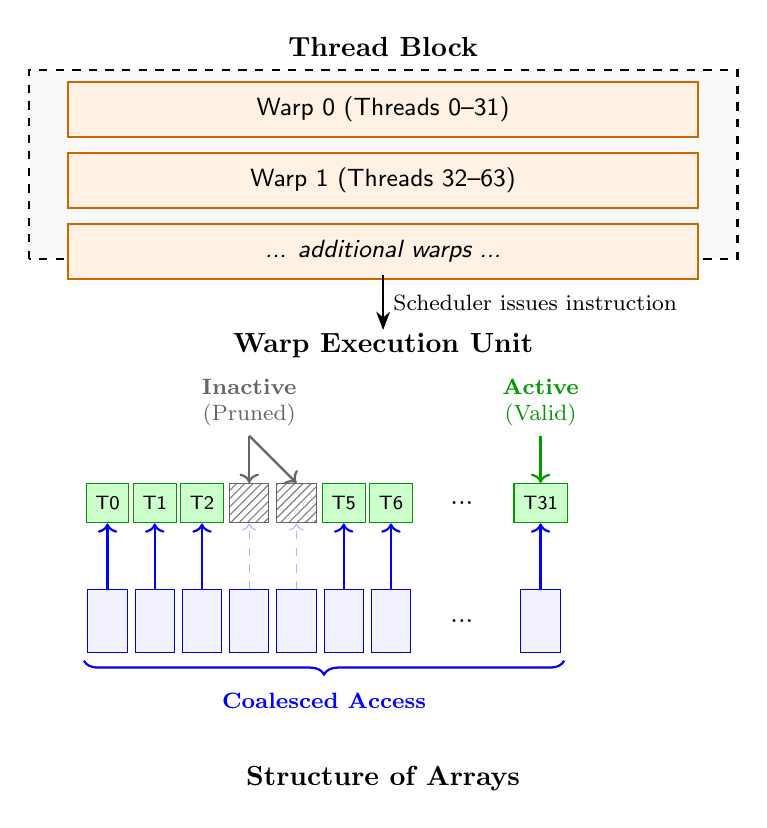
\begin{tikzpicture}[
        warp/.style={
            rectangle, 
            draw=orange!80!black, 
            fill=orange!10, 
            thick, 
            minimum width=8cm, 
            minimum height=0.7cm, 
            font=\small\sffamily
        },
        thread_active/.style={
            rectangle, 
            draw=green!60!black, 
            fill=green!20, 
            minimum size=0.5cm, 
            font=\scriptsize\sffamily
        },
        thread_inactive/.style={
            rectangle, 
            draw=gray!80!black, 
            fill=gray!20, 
            minimum size=0.5cm, 
            pattern=north east lines, 
            pattern color=gray,
            font=\scriptsize\sffamily
        },
        mem_cell/.style={
            rectangle,
            draw=blue!80!black,
            fill=blue!5,
            minimum width=0.5cm,
            minimum height=0.8cm,
            font=\tiny
        }
    ]

    \node (block_label) at (0, 5.8) {\textbf{Thread Block}};

    \draw[thick, dashed, fill=gray!5] (-4.5, 3.1) rectangle (4.5, 5.5);
    

    \node (warp0) [warp] at (0, 5.0) {Warp 0 (Threads 0--31)};
    \node (warp1) [warp] at (0, 4.1) {Warp 1 (Threads 32--63)};
    \node (warp2) [warp] at (0, 3.2) {\textit{... additional warps ...}};

    \node (simt_label) at (0, 2.0) {\textbf{Warp Execution Unit}};
    

    \draw [->, thick, >=Stealth] (0, 2.9) -- (0, 2.2) node[midway, right, font=\footnotesize] {Scheduler issues instruction};

    \node (t0) [thread_active] at (-3.5, 0) {T0};
    \node (t1) [thread_active] at (-2.9, 0) {T1};
    \node (t2) [thread_active] at (-2.3, 0) {T2};

    \node (t3) [thread_inactive] at (-1.7, 0) {};
    \node (t4) [thread_inactive] at (-1.1, 0) {};
    
    \node (t5) [thread_active] at (-0.5, 0) {T5};
    \node (t6) [thread_active] at (0.1, 0) {T6};
    
    \node at (1.0, 0) {...};
    \node (t31) [thread_active] at (2.0, 0) {T31};

    \node (lbl_active) [above=0.6cm of t31, font=\footnotesize, color=green!60!black, align=center] {\textbf{Active}\\(Valid)};
    \draw [->, thick, green!60!black] (lbl_active.south) -- (t31.north);

    \node (lbl_inactive) [above=0.6cm of t3, font=\footnotesize, color=gray!80!black, align=center] {\textbf{Inactive}\\(Pruned)};
    \draw [->, thick, gray!80!black] (lbl_inactive.south) -- (t3.north);
    \draw [->, thick, gray!80!black] (lbl_inactive.south) -- (t4.north);

    \node (mem_label) at (0, -3.5) {\textbf{Structure of Arrays}};
    
    \foreach \x [count=\i] in {-3.5, -2.9, -2.3, -1.7, -1.1, -0.5, 0.1} {
        \node [mem_cell] (m\i) at (\x, -1.5) {};
    }
    \node at (1.0, -1.5) {...};
    \node [mem_cell] (m31) at (2.0, -1.5) {};

    \draw [->, blue, thick] (m1.north) -- (t0.south);
    \draw [->, blue, thick] (m2.north) -- (t1.south);
    \draw [->, blue, thick] (m3.north) -- (t2.south);
    
    \draw [->, blue!30, dashed] (m4.north) -- (t3.south);
    \draw [->, blue!30, dashed] (m5.north) -- (t4.south);
    
    \draw [->, blue, thick] (m6.north) -- (t5.south);
    \draw [->, blue, thick] (m7.north) -- (t6.south);
    \draw [->, blue, thick] (m31.north) -- (t31.south);

    \draw [decorate, decoration={brace, amplitude=5pt, mirror}, thick, blue] (-3.8, -2.0) -- (2.3, -2.0) node [midway, below=8pt, font=\footnotesize, color=blue, align=center] {\textbf{Coalesced Access}\\};

    \end{tikzpicture}
    

\end{document}
